\chapter{Modern Physics}

\pagestyle{fancy}
\fancyhf{}
\fancyhead[OC]{\leftmark}
\fancyhead[EC]{\rightmark}
%\renewcommand{\footrulewidth}{1pt}
\cfoot{\thepage}

\section{Key Concepts and Formulae}
\subsection{Relativity}
\begin{enumerate}
\item \textbf{Proper Length:} It is the length of the body along the moving direction measured by an observer in his frame of reference.
\item \textbf{Proper Time:} It the time measured by an observer in his frame of reference by using his own clock.
\item Lorentz factor ($\gamma$) is given by
\begin{align}
    {\gamma} = \dfrac{1}{\sqrt{1-\dfrac{v^2}{c^2}}}     \label{eq1}
\end{align}
\item Total energy of a relativistic particle is related as:
\begin{align}
E^2  =  P^2C^2  +  {M_o}^2C^4      \label{eq2}
\end{align}
\item Momentum of relativistic particle,
\begin{align}
P = {\gamma}{M_o}v      \label{eq3}
\end{align}
\item Generally, we use K-frame or S-frame to denote inertial frame or laboratory frame where the body is at rest and k'-frame or S'-frame to denote the moving one.
\end{enumerate}
\subsection{Quantum Mechanics}
\begin{enumerate}
    \item De Broglie wavelength: $\lambda$ = $\dfrac{2 \pi \hbar}{p}$, where p is the momentum of the particle. 
    \item \textbf{Uncertainty Relations}: 
    \begin{align}
        \text{position- linear momentum }\Delta p \Delta x \geq \hbar \\
        \text{Energy-time }\Delta E \Delta t \geq \hbar\\
        \text{angular momentum - angle }\Delta L \Delta \theta \geq \hbar
    \end{align}
    \item \textbf{Schrodinger's wave equation:}\\
    one-dimensional time dependent equation: 
    \begin{align} 
        i\hbar\dfrac{\partial \Psi}{\partial t} = - \dfrac{\hbar ^2}{2m}\dfrac{\partial ^2 \Psi}{\partial x^2} + U \Psi
    \end{align}
    one-dimensional time independent equation: 
    \begin{align}
        \dfrac{\partial^2 \psi}{\partial x^2} + \dfrac{2m}{\hbar ^2}(E- U)\psi = 0
    \end{align}
    Here $\Psi$ is a time dependent wave function generally represented as $\Psi(x,t)$ in 1-D. And $\psi$ is time-independent or coordinate part of $\Psi (x, t)$. 
    
    \item Free particle: When U(x) = 0, we generally call it free. In such case, the Schrodinger's equation becomes: 
    \begin{align*}
        \psi(x) = Ae^{ikx}E = \dfrac{\hbar^2 k^2}{2m}
    \end{align*}
    \item Particle in a Box: If there is a non-zero potential wall, we call it a box.  
\end{enumerate}
\section{Bridging Problems}

\begin{enumerate}

\item A Russian physicist P.A. Cerenkov discovered that a charged particle travelling in a solid at the speed of light in that material radiates electromagnetic radiation. What is the minimum kinetic energy in eV that an electron must have while travelling inside a slab of crown glass of refractive index 1.52 in order to create Cerenkov radiation? \hfill \textsl{(NePhO, UP)}

\textsc{Solution:}\\
For an electron of mass ‘m’ and charge ‘e’,\\
Inside the slab, the velocity of light can be calculated as,
\begin{align*}
v = \frac{c}{\mu}
\end{align*}
Then Kinetic Energy is given by,
\begin{align*}
    K.E.&= \left(\mu-1\right)mc^2\\
    &= \left(\ddfrac{1}{\sqrt{1-\frac{v^2}{c^2}}}-1\right)mc^2 \hspace{1cm} \text{Using \eqref{eq1}}
\end{align*}
Solving we get,
\[
K.E._{min}= 0.168 MeV
\]

\item A particle of mass m moves in a one-dimensional potential
\[
V(x) = A\mathopen|x\mathclose|,\hspace{1cm} \text{where A is a positive constant.}
\]
Use the Heisenberg uncertainty principle to estimate the minimum total energy of the particle as a function of m, A, and $\hbar$.\hfill \textsl{(NePhO)}
\\
\textbf{Solution:}\\
One-dimensional potential is given by,
\begin{align*}
V(x) &= A\mathopen|x\mathclose|      \label{eq4}\\
\text{Total Energy(T.E.)} &= \text{K.E. + P.E.}\\
&= \dfrac{p^2}{2m} + mA\mathopen|x\mathclose|
\end{align*}
from uncertainty principle, $\Delta$p $\times \Delta$x $\geq$ $\frac{\hbar}{2\pi}$\\
\begin{align*}
    \text{hence, P } &= \frac{\hbar}{2\pi x} \text{and, }\\
    E &= \frac{\hbar^2}{8m\pi^2x^2} +  mAx 
\end{align*}
For 'E' to be minimum, 
\begin{align*}
    \dfrac{dE}{dx} &= 0\\
    \text{or, }mA &=  \frac{\hbar^2}{4m\pi^2x^3}\\
    \text{or, }x &= \left(\frac{\hbar^2}{4m^2A\pi^2}\right)^\frac{1}{3}\\
\end{align*}
Hence, \\
\[E_{min} = \]

\item The smallest length scale one can resolve is called the Planck Length $L_p$, which can be estimated in the following way. To get information within the length scale $L$, one needs a photon with the wavelength $\lambda$ roughly the same as the length scale. But any photon creates a (tiny) blackhole within which no information can get out. When the photon wavelength is equal 2 times the radius of the blackhole ($=L_p$), then we obtain the smallest length scale $L_p$. Note that a photon with wavelength $\lambda$ has energy $E = hc/\lambda$ and effective mass $m = E/c^2$. 
\begin{enumerate}
    \item Determine the Planck length.
    \item Determine the Planck energy $E_p$ which is the energy of a photon with its wavelength equal to $2\pi$ times the Planck length, in terms of electron volts(eV). You may find the constant hc = 1240eV.nm useful. 
\end{enumerate}
\hfill \textsl{(HKPhO)}\\
\textbf{Solution:}\\
a) \\
From given information, we know, \\
\begin{align}
    \lambda_p &= 2\pi L_p \\
    m &= \frac{E}{c^2}
\end{align}
Schwarzschild's radius in this case is: 
\begin{align}
    L_p  &= \frac{2Gm}{c^2}\\
    \text{and, }E &= \frac{hc}{\lambda}
\end{align}
Using above relations, we get: \\
\begin{align*}
    \frac{hc}{E}  &=  2\pi L_p \\
    \text{or, }\frac{hc}{mc^2}   &=   2\pi L_p\\
    \text{or, }\frac{2Gh}{c^3}  &=  2\pi L^2_p\\
    \therefore L_p &= \sqrt{\frac{Gh}{c^3\pi}}
\end{align*}
b) \\
\begin{align*}
    E_p &= \frac{hc}{\lambda_p}\\
    E_p &= \frac{hc}{2\pi L_p}
\end{align*}
Substituting 'L$_p$' from (a), we get:
\begin{align*}
    E_p &= \sqrt{\dfrac{hc^5}{4\pi G}}\hspace{2cm}Q.E.D.
\end{align*}
\item Consider a hydrogen atom of an electron bound to a proton. The system of electron and proton has, kinetic energy, $K = \ddfrac{P^2}{2m}$ , potential energy $U = -\ddfrac{ke^2}{r}$ , and total energy $E = K + U$. Treat the atom as a one dimensional system. The system will be stable when its total energy is minimum. By minimizing the total energy, estimate the radius of the atom and resulting total energy. \\
\textbf{Solution:}\\
\begin{align*}
    E = \dfrac{p^2}{2m} - \dfrac{ke^2}{r}
\end{align*}
Also, p $\sim \Delta$p and r $\sim \Delta$r\\
By Uncertainty Principle, $\Delta$p$\Delta$r $\sim \hbar$
\begin{align*}
    E &= \dfrac{p^2}{2m} - \dfrac{ke^2}{r}\\
    E &=  \frac{1}{2m}\dfrac{\hbar^2}{r^2}  - \frac{ke^2}{r}
\end{align*}
Fr E to be minimum, 
\begin{align*}
    \dfrac{dE}{dr} &= 0\\
    \text{or, } \frac{ke^2}{r^2}   &= \dfrac{\hbar^2}{m r^3}\\
    \text{or, }r   &=   \frac{\hbar^2}{mke^2}
\end{align*}
Putting the value of ‘r’ we get,  \\
\[E_{min.}  =  -\dfrac{mk^2e^4}{2\hbar^2} \]
\\
\item A particle of rest mass $m_o$ and speed $v$ collides with a stationary particle of mass $M$ and sticks to it. What is the final speed of the composite particle?\\

\textbf{Solution:}\\

Let M$_c$ be the mass of the composite particle and $\gamma_c$ be the factor, and ‘u’ be the speed. This is an inelastic collision where kinetic energy is not conserved. But be careful, the total energy and also the momentum are conserved.\\
By conservation of momentum, \\
\begin{align}
    \gamma m_o v  &= \gamma_c M_c u   
\end{align}
And, from conservation of total energy,
\begin{align}
    \gamma m_o c^2  +  Mc^2  &=  \gamma_c M_c c^2
\end{align}
from eqn 5.8 and 5.9, 
\begin{align*}
    \text{or, }\gamma m_o   +  M  &=  \frac{\gamma m_o v}{u}\\
    \therefore u &=  \frac{\gamma m_ov}{\gamma m_o + M}
\end{align*}
\end{enumerate}

\section{Level 1 Problems and Solutions}
\begin{enumerate}
\item The ground state wave function of an hydrogen atom(in 1s state) is
\begin{align}
\Psi_{1s} = \frac{1}{\sqrt{\pi a^3}}e^{-x/a}   \label{eq4}
\end{align}
Show that the probability of finding the electron over all space is one. \hfill \textsl{(UP)}
\textbf{Solution:}\\
\[
\text{!!!!! SOLUTION !!!!!}
\]
\item Neutrinos are very light particles with masses below 10 eV. Estimate the speed of a neutrino with total energy of 108 eV in the unit of the speed of light in vacuum \emph{c}.

\textsc{Solution:}\\
\[
\text{!!!!! SOLUTION !!!!!}
\]

\item When studying problems in special relativity it is often the invariant distance $\Delta s$ between two events that is most important, where $\Delta s$ is defined by
\begin{align}
(\Delta s)^2 = (c \Delta t)^2 - [(\Delta x)^2 + (\Delta y)^2 + (\Delta z)^2]   \label{eq5}
\end{align}
where, $c = 3\times10^8$ m/s is the speed of light.
\begin{enumerate}
    \item Consider the motion of a projectile launched with initial speed $V_{o}$ at angle of $\theta^\circ$ above the horizontal. Assume that g, the acceleration of free fall, is constant for the motion of the projectile.
\end{enumerate}

\textsc{Solution:}\\
\[
\text{!!!!! SOLUTION !!!!!}
\]

\item A particle of rest mass $m_o$ and kinetic energy $x{m_o}c^2$, where $x$ is some number, strikes an identical particle at rest and sticks to it. What is the rest mass of the resultant particle?

\textsc{Solution:}\\
\[
\text{!!!!! SOLUTION !!!!!}
\]

\end{enumerate}

\section{Level 2 Problems and Solutions}

\begin{enumerate}
\item We define three quantities as follow:
\[
A = {m_e}c^2,\hspace{0.5cm} B = h/{m_e}c,\hspace{0.5cm} C = e^2/2{\epsilon_0}ch
\]
Where $m_e$ is electron mass and other symbols have their usual meanings. For the hydrogen atom, express the radius of the $n^{\text{th}}$ Bohr orbit $r_n$ , energy level $E_n$, and the Rydberg constant R in terms of any two of \{A, B, C\} \hfill \textsl{(InPhO 2008)}

\textsc{Solution:}\\
\[
\text{!!!!! SOLUTION !!!!!}
\]

\item The mass of an electron at rest, in the unit of energy using the mass-energy equivalence relation, is $0.511 \times 106 eV$, or 0.511 $MeV$, and $eV$ is electron-Volt. Find the momentum of an electron, in the unit of $MeV/c$ ($c$ is the speed of light in vacuum and keep only two digits) when its kinetic energy is
\begin{enumerate}
    \item $1.0 \times 10^{-6} MeV$
    \item $1.0 MeV$
    \item $1.0 \times 10^{6} MeV$
\end{enumerate}

\textsc{Solution:}\\
\[
\text{!!!!! SOLUTION !!!!!}
\]

\item Find the deBroglie wavelength of:
\begin{enumerate}
    \item an electron with kinetic energy of 1 eV
    \item an electron with kinetic energy of 10 MeV
    \item a neutron with kinetic energy of 10 MeV
    \item a 500 g grapefruit that has been thrown with a speed of 10 m/s
\end{enumerate}

\begin{note}
Make sure to consider whether you need to use relativistically correct equations in each case!
\end{note}

\textsc{Solution:}\\
\[
\text{!!!!! SOLUTION !!!!!}
\]

\item \begin{enumerate}
    \item Two particles of rest mass $m$ approach each other with equal and opposite velocity, $u$, as measured in the lab frame. What is the total energy of one particle as measured in the rest frame of the other? Express your answer in terms of $u$ and $m$.
    
    \item Express your answer from part (a) in terms of the initial total energy of each particle.
    
    \item Suppose the two particles are protons ($mc^2 \approx 1 GeV$), each with an initial total energy of $30 GeV$. What is the energy of one proton as measured in the rest frame of the other?

\textsc{Solution:}\\
\[
\text{!!!!! SOLUTION !!!!!}
\]

\end{enumerate}
\item In the Compton effect, a $\gamma$-ray photon of wavelength $\lambda$ strikes a free, but initially stationary, electron of mass m. The photon is scattered an angle $\theta$ and its scattered wavelength is $\Tilde{\lambda}$. The electron recoils at an angle $\phi$.
\begin{figure}[htp]
    \centering
    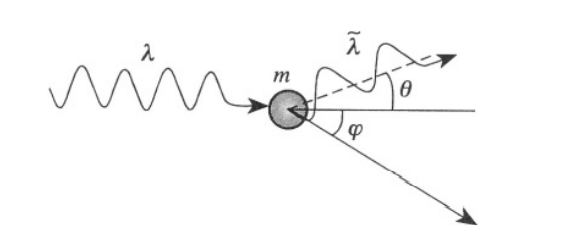
\includegraphics{mainmatter/wave2.PNG}
    \caption{}
    \label{fig:my_label}
\end{figure}
\begin{enumerate}
    \item Write the relativistic equations for momentum and energy conservation.
    \item Find an expression for the change $\lambda$ - $\Tilde{\lambda}$ in the photon wavelength for special case $\theta$ = $\pi$/2. 
\end{enumerate}
\item 
\end{enumerate}